% EDIA -- IEEE conference paper draft (IEEEtran). Compile on Overleaf or any TeX
% distribution with IEEEtran:  pdflatex edia_ieee && bibtex edia_ieee && pdflatex x2
% Every number below is traced to a committed file; see paper/NUMBERS.md.
\documentclass[conference]{IEEEtran}
\IEEEoverridecommandlockouts
\usepackage{cite}
\usepackage{amsmath,amssymb}
\usepackage{graphicx}
\usepackage{booktabs}
\usepackage{multirow}
\usepackage{xcolor}
\usepackage{url}
\usepackage{textcomp}

% Draft markers -- every \TODO must be resolved (or removed) before submission.
\newcommand{\TODO}[1]{\textcolor{red}{[TODO: #1]}}

\begin{document}

\title{Where Meeting Reasoning Gets Lost: A Feasibility Study of\\
Decision-Context Gap Detection in Enterprise Meetings}

\author{\IEEEauthorblockN{Jaitra Shah}
\IEEEauthorblockA{\TODO{Department} \\
\TODO{Institution}\\
\TODO{City, Country} \\
\TODO{email}}
\and
\IEEEauthorblockN{\TODO{Co-author / supervisor}}
\IEEEauthorblockA{\TODO{Department} \\
\TODO{Institution}\\
\TODO{City, Country} \\
\TODO{email}}
}

\maketitle

\begin{abstract}
Meetings produce decisions, but the reasoning behind them---alternatives weighed,
rationale, conditions and dissent---rarely survives into the written record. We
study whether current AI can recover that reasoning and detect when a filed
document has dropped it. We build EDIA, a pipeline that extracts structured
decision reasoning from transcripts with an open 7B language model and flags
reasoning elements missing from the accompanying document, and we evaluate it on
\textit{adhd\_v1}, a 371-pair, 6{,}647-element benchmark with three label tiers
(hand-labelled, NLI-labelled, and constructed). Three findings stand out. First,
on the only class-balanced tier a lexical-overlap detector outperforms an NLI
entailment detector (balanced accuracy 0.775 vs.\ 0.629), because NLI fails to
recognise content that \emph{did} survive into a compressed summary, including
verbatim copies (accuracy 0.292); an LLM judge performs at chance, and a human
spot-check finds that about half of the gaps flagged by NLI-produced corpus
labels are content the summary does contain. Second,
extraction recovers 33.3--58.3\% of human-identified reasoning (lexical to
semantic matching) on hand-labelled meetings, and 55\% of the residual misses
require multi-hop reasoning across distant turns, while none are caused by
chunk boundaries. Third, chain-of-thought prompting, GraphRAG and multi-hop
retrieval do not lift this ceiling (GraphRAG: 4.2--14.6\%). We argue the ceiling
is structural: the missing reasoning is scattered and implicit, which current
retrieval and generation methods do not address.
\end{abstract}

\begin{IEEEkeywords}
meeting summarization, decision extraction, natural language inference,
information extraction, multi-hop reasoning, evaluation
\end{IEEEkeywords}

% ---------------------------------------------------------------------------
\section{Introduction}

Organisations record \emph{what} was decided far more reliably than \emph{why}.
Minutes and summaries compress hours of discussion into a few sentences, and the
reasoning that made a decision defensible---which options were rejected, which
concerns were raised, which conditions were attached---is the first thing cut.
When that reasoning is later needed, for an audit, a reversal, or onboarding, it
is often gone. We call a reasoning element that was voiced in a meeting but is
absent from the filed document a \emph{decision-context gap}.

Detecting such gaps automatically requires two capabilities: extracting the
reasoning that a meeting actually contains, and deciding whether each extracted
element is present in the document. Both look within reach of current language
models. This paper tests that assumption rigorously rather than assuming it, and
reports where and why it breaks.

We make four contributions:
\begin{itemize}
\item \textbf{EDIA}, an end-to-end pipeline for structured decision-reasoning
extraction and gap detection, run entirely on open models.
\item \textbf{adhd\_v1}, a three-tier benchmark (hand-labelled, NLI-labelled and
constructed pairs) with explicit label provenance, designed so that detector
comparisons are made where the class balance allows them to be meaningful.
\item \textbf{A diagnosis} of the extraction ceiling through a manually
annotated failure taxonomy, showing that multi-hop reasoning---not chunking,
paraphrase or hallucination---dominates the residual misses.
\item \textbf{A comparative analysis} showing that chain-of-thought prompting,
GraphRAG and multi-hop retrieval each fail to break the ceiling for an
identifiable reason.
\end{itemize}

Our answer to the feasibility question is \emph{partially}: the pipeline recovers
roughly a third to a half of the reasoning a human finds, and the remainder is
precisely the reasoning that is hardest to locate.

% ---------------------------------------------------------------------------
\section{Background and Related Work}

\textbf{Meeting corpora and summarization.} QMSum~\cite{zhong2021qmsum} pairs
meeting transcripts from three domains---academic group meetings from the ICSI
corpus~\cite{janin2003icsi}, product-design meetings from the AMI
corpus~\cite{carletta2005ami}, and parliamentary committee meetings---with
query-based summaries. We use QMSum's summaries as stand-ins for filed documents:
they are exactly the kind of compressed, human-written record in which
reasoning is lost.

\textbf{Entailment for faithfulness.} Natural language inference (NLI) models
trained on MNLI~\cite{williams2018mnli}, such as RoBERTa-large~\cite{liu2019roberta},
are widely used to test whether a summary is supported by its source, e.g.\
SummaC~\cite{laban2022summac} and FactCC~\cite{kryscinski2020factcc}. Gap
detection inverts that direction: the question is whether a \emph{source} element
is carried by a much shorter summary, which we find to be a poor fit for
sentence-level NLI.

\textbf{LLMs as judges.} Using a language model to grade content is attractive
but known to suffer from systematic biases~\cite{zheng2023judging}; we observe a
severe instance.

\textbf{Retrieval and multi-hop reasoning.} Retrieval-augmented
generation~\cite{lewis2020rag} and multi-hop question answering~\cite{yang2018hotpotqa}
address evidence spread across documents. GraphRAG~\cite{edge2024graphrag}
builds an entity graph with community summaries for query-focused summarization.
Chain-of-thought prompting~\cite{wei2022cot} improves reasoning over content
already in context. None is designed for reasoning that is scattered across a
long, multi-speaker conversation and often never stated explicitly.

% ---------------------------------------------------------------------------
\section{The EDIA Pipeline}

Fig.~\ref{fig:pipeline} summarises the pipeline: transcripts are chunked and
passed to an extractor that emits structured decision records, whose reasoning
elements are then checked against the filed document by a gap detector.

\begin{figure}[t]
\centering
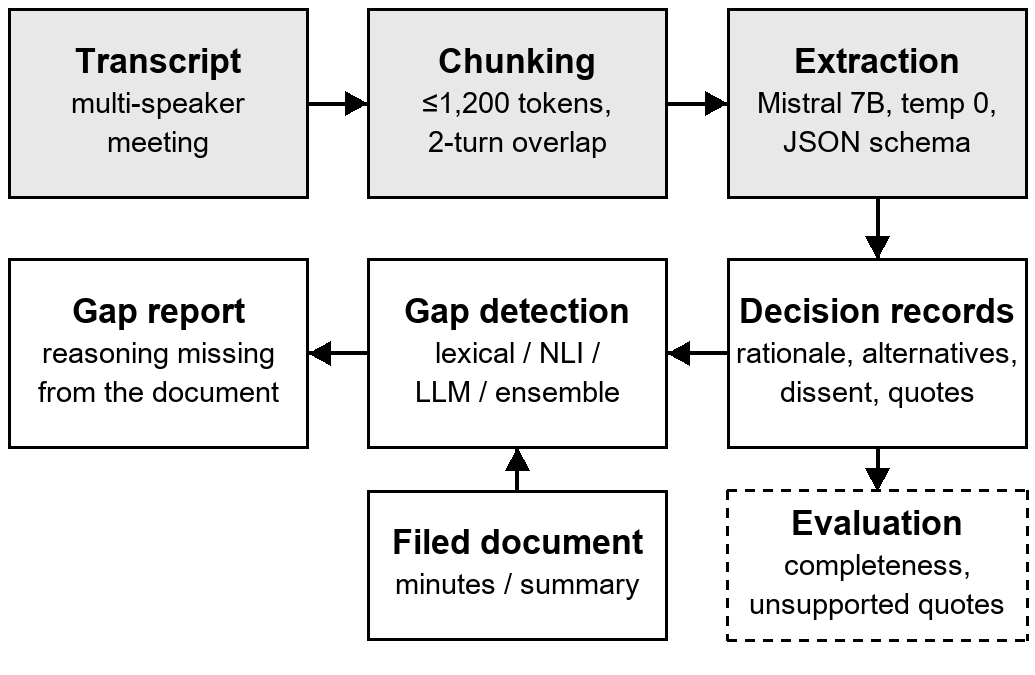
\includegraphics[width=\columnwidth]{fig_pipeline.png}
\caption{The EDIA pipeline. Grey: extraction stage; dashed: evaluation. In the
benchmark, gap detectors are scored directly on labelled reasoning elements, and
extraction is scored separately against hand-labelled ground truth.}
\label{fig:pipeline}
\end{figure}

\subsection{Schema and extraction}
Each decision is represented as a record with the decision statement, topic,
status (decided, provisional, deferred, rejected, unclear), alternatives
(with rejection flag and reason), rationale, conditions, dissent, owner,
approver, and verbatim evidence quotes with speaker labels. Transcripts are
split into chunks of at most 1{,}200 tokens with a two-turn overlap, and each
chunk is sent to Mistral~7B~\cite{jiang2023mistral} (via Ollama\footnote{\url{https://ollama.com}})
with a prompt that forbids inference beyond the excerpt and requires quotes to
be copied character-for-character. Decoding settings are deterministic
(temperature~0, top-$k$~1, fixed seed, 8{,}192-token context, 2{,}048-token output
cap) under JSON-constrained output; unparseable output triggers one repair call.

\subsection{Gap detection}
Given a document and a reasoning element, a detector returns a present-score in
$[0,1]$; the element is predicted to be a gap if the score is below a threshold
(0.55). We compare four detectors: (i)~\emph{lexical}, token-level F1 overlap
with the document; (ii)~\emph{NLI}, the entailment probability of the element
given the document under \texttt{roberta-large-mnli}; (iii)~an \emph{LLM judge},
Mistral~7B asked whether the substance of the element is present in the
document, returning a verdict and confidence; and (iv)~an \emph{ensemble} that
shifts each member's present-score by that member's own threshold (so that 0.5
means ``present'' for every member) and takes the maximum, i.e.\ it calls an
element present if any member does.

\subsection{Evaluation design}
\textbf{The base-rate problem.} Most elements in real summaries are gaps: in the
NLI-labelled QMSum tier the gap rate is 0.93, where a detector that answers
``gap'' to everything obtains a gap-class F1 of about 0.96. Gap F1 alone is
therefore nearly uninformative. We report \emph{balanced accuracy} (the mean of
gap and present recall, 0.5 for any constant detector) and \emph{present-class F1}
beside every gap F1, and make detector comparisons on the class-balanced
synthetic tier.

\textbf{Completeness.} Extraction is scored as the fraction of hand-labelled
reasoning elements matched by some extracted element. Because correct
extractions are often worded differently, we report two matchers and never one
alone: \emph{lexical} (token F1 $\geq$ 0.45) and \emph{semantic} (cosine
similarity of all-MiniLM-L6-v2 sentence embeddings~\cite{reimers2019sbert}
$\geq$ 0.55).

\textbf{Hallucination.} Each evidence quote is checked against its own source
chunk after normalising case, punctuation and whitespace, and additionally
ignoring transcription markers and filler words. The \emph{unsupported-quote
rate} is the fraction of quotes not found under this check.

% ---------------------------------------------------------------------------
\section{Dataset: adhd\_v1}

Table~\ref{tab:dataset} summarises the benchmark. Each pair contains a
transcript, a short document, reasoning elements, and a per-element label:
\emph{omitted} (a gap), \emph{verbatim}, \emph{paraphrased}, or present with
unspecified wording.

\begin{table}[t]
\caption{The adhd\_v1 benchmark (dataset locked).}
\label{tab:dataset}
\centering
\small
\begin{tabular}{@{}lrrrl@{}}
\toprule
Tier & Pairs & Elements & Gap rate & Labels \\
\midrule
Gold (QMSum) & 5 & 50 & 0.76 & human \\
Corpus (QMSum) & 227 & 4{,}930 & 0.93 & NLI @ 0.55 \\
Synthetic & 139 & 1{,}667 & 0.59 & constructed \\
\midrule
Total & 371 & 6{,}647 & 0.84 & \\
\bottomrule
\end{tabular}
\end{table}

\textbf{Gold.} Five QMSum product-design meetings, hand-labelled against
transcript spans. They are the trust anchor and the only meetings with
reasoning ground truth for completeness scoring; with $n=5$ and one domain they
are a fixture, not an accuracy estimate.

\textbf{Corpus.} All other 227 QMSum meetings (Academic 59, Committee 36,
Product 132), with summaries split into 4{,}930 sentence-level elements labelled
by the NLI detector at threshold 0.55, chosen on the gold pairs. These are
\emph{silver} labels: scoring the NLI detector against them measures
self-consistency, not accuracy, and we exclude that comparison.

\textbf{Human spot-check of the silver labels.} One author judged 52 elements
from three randomly sampled corpus pairs (two Academic, one Committee), blind to
the silver labels. The silver labels never missed a gap the annotator saw
(gap recall 1.0), but 24 of their 46 predicted gaps were judged present in the
summary, 23 of them as paraphrases (gap precision 0.478, present recall 0.20,
balanced accuracy 0.60). The direction of the error is consistent across all
three pairs, although 19 of the 24 disagreements come from the Committee
pair. The silver labels therefore substantially overstate the gap rate, in line
with NLI's weakness on paraphrased content reported in Section~V, and corpus-tier
figures should be read as upper bounds on the gap rate.

\textbf{Synthetic.} 139 pairs generated by Mistral~7B across 12 organisational
domains and 10 decision archetypes. Labels are \emph{constructed}: each
element's fate (omitted, verbatim, paraphrased) is fixed before either text is
written, followed by an automated leak check. This is the only tier with a
near-balanced gap rate, which is why detector comparisons are made on it.
Synthetic transcripts are cleaner than real meetings, which we treat as a
limitation.

% ---------------------------------------------------------------------------
\section{Results: Gap Detection}

\begin{table}[t]
\caption{Gap detection at threshold 0.55. The NLI-labelled corpus tier is omitted
for NLI (circular). Bal.\ acc.\ = balanced accuracy.}
\label{tab:detect}
\centering
\small
\begin{tabular}{@{}llrrrr@{}}
\toprule
Detector & Tier & $n$ & Gap F1 & Bal.\ acc. & Pres.\ F1 \\
\midrule
NLI & gold & 50 & 0.861 & 0.656 & 0.476 \\
NLI & synthetic & 1{,}667 & 0.771 & 0.629 & 0.468 \\
Lexical & gold & 50 & 0.884 & 0.583 & 0.286 \\
Lexical & synthetic & 1{,}667 & 0.857 & \textbf{0.775} & \textbf{0.715} \\
Lexical & corpus & 4{,}930 & 0.970 & 0.669 & 0.457 \\
\midrule
\multicolumn{6}{@{}l}{\textit{Same stratified sample, gold + synthetic ($n=200$)}} \\
NLI & & 200 & -- & 0.611 & 0.432 \\
Lexical & & 200 & -- & \textbf{0.728} & \textbf{0.637} \\
LLM judge & & 200 & -- & 0.492 & 0.596 \\
Ensemble & & 200 & -- & 0.521 & 0.624 \\
\bottomrule
\end{tabular}
\end{table}

Table~\ref{tab:detect} reports the comparison. On the balanced synthetic tier,
the lexical detector outperforms NLI on every honest metric (balanced accuracy
0.775 vs.\ 0.629; present F1 0.715 vs.\ 0.468). The same ordering holds when all
four detectors are scored on one shared stratified sample of 200 gold and
synthetic elements.

\textbf{NLI cannot see content that survived.} Broken down by label on the
gold and synthetic tiers (excluding NLI's own corpus labels), NLI identifies
true gaps well (accuracy 0.916; lexical 0.974) but recognises paraphrased-present
elements only 36.6\% of the time and verbatim-present elements only 29.2\% of
the time (lexical: 64.0\% and 45.3\%). A detector that misses literal copies is not
performing entailment in any useful sense: against a compressed summary of about
100 words, almost every source sentence reads as not entailed. A consequence is
that the NLI-labelled corpus tier overstates its gap rate, so corpus-tier
figures are best read as an upper bound.

\textbf{The LLM judge is at chance.} On a 296-element stratified sample, the
Mistral~7B judge labelled about 95\% of elements as present, including obvious
omissions, for a gap recall of 0.047 and balanced accuracy of 0.495; the ensemble,
which calls an element present if any member does, inherits this bias (0.516 at
the common 0.55 threshold; at its designed 0.5 operating point it labels every
sampled element present). We verified
that the judge received the short summaries and correct labels, so this is a
genuine yes-bias under a fixed prompt, consistent with known LLM-judge
biases~\cite{zheng2023judging}, and not a pipeline error.

\textbf{Base-rate distortion.} Per-domain lexical results on the corpus tier show
why gap F1 misleads: Committee meetings give the highest gap F1 of any bucket
(0.988) and the lowest balanced accuracy (0.532), because their summaries are
almost entirely meta-description and guessing ``gap'' wins.

% ---------------------------------------------------------------------------
\section{Results: Extraction and Its Ceiling}

\begin{table}[t]
\caption{Extraction completeness on the five hand-labelled meetings.}
\label{tab:complete}
\centering
\small
\begin{tabular}{@{}lrr@{}}
\toprule
Meeting & Lexical & Semantic \\
\midrule
QSUM\_001 & 0.455 & 0.636 \\
QSUM\_002 & 0.500 & 0.875 \\
QSUM\_003 & 0.111 & 0.222 \\
QSUM\_004 & 0.286 & 0.643 \\
QSUM\_005 & 0.333 & 0.500 \\
\midrule
Pooled & \textbf{0.333} (16/48) & \textbf{0.583} (28/48) \\
\bottomrule
\end{tabular}
\end{table}

\textbf{Completeness is a range.} On the gold meetings EDIA recovers 33.3\%
(lexical) to 58.3\% (semantic) of the hand-labelled reasoning
(Table~\ref{tab:complete}). The gap between the two matchers is itself a
finding: 14 of the 32 lexical misses are correct extractions that token overlap
under-credits (e.g.\ the headline decision ``Kryptonite was chosen as the
preferred energy source'' scores 0.36), so the lexical figure is a floor. The
unsupported-quote rate on these meetings is 16.4\%.

\begin{table}[t]
\caption{Corpus-wide extraction (227 meetings): unsupported-quote rate by domain.
``Tidied'' = unsupported quotes whose words all appear, in order, in the source
chunk (words dropped, none added).}
\label{tab:corpus}
\centering
\small
\begin{tabular}{@{}lrrrr@{}}
\toprule
Domain & Meetings & Quotes & Unsupp. & Excl.\ tidied \\
\midrule
Academic & 59 & 6{,}341 & 26.7\% & 7.6\% \\
Committee & 36 & 5{,}441 & 5.1\% & 3.6\% \\
Product & 132 & 10{,}167 & 12.0\% & 5.1\% \\
\midrule
All & 227 & 21{,}949 & 14.6\% & 5.4\% \\
\bottomrule
\end{tabular}
\end{table}

\textbf{Grounding across domains.} Completeness cannot be measured outside the
gold meetings, but grounding can. Table~\ref{tab:corpus} reports the
unsupported-quote rate over all 227 corpus meetings (3{,}532 chunks; 36, or 1.0\%,
failed because the model entered a repetition loop). Academic meetings appear
far worse (26.7\%), but 72\% of their unsupported quotes are near-verbatim: the
model drops the false starts, repetitions and word fragments that are pervasive
in ICSI speech. Excluding such tidying, the three domains fall within
3.6--7.6\%, indicating that the extractor behaves consistently across domains.
We report the stricter figure as the hallucination rate.

\begin{table}[t]
\caption{Failure taxonomy of the 20 semantic-residual misses, from manual reading
of the transcript evidence for each miss.}
\label{tab:taxonomy}
\centering
\small
\begin{tabular}{@{}lrr@{}}
\toprule
Failure category & $n$ & Share \\
\midrule
Multi-hop, implicit (connection never stated) & 6 & 30\% \\
Multi-hop, scattered (turns far apart) & 5 & 25\% \\
Paraphrase miss (scorer did not match) & 5 & 25\% \\
Out of scope (local, not extracted) & 4 & 20\% \\
Chunk boundary & 0 & 0\% \\
Hallucination & 0 & 0\% \\
\bottomrule
\end{tabular}
\end{table}

\textbf{Why the ceiling exists.} Table~\ref{tab:taxonomy} categorises every
residual miss by manually reading where its supporting content sits in the
transcript. Multi-hop reasoning accounts for 11 of 20 misses (55\%): the
reasoning is either spread across turns far apart---in one meeting, about 670
turns separate the two halves of a single rationale---or never stated
explicitly and must be inferred. The zeros matter as much: no miss was caused
by a chunk cut, so a longer context window would not address these failures,
and no miss was caused by a fabricated quote, so the misses are omissions rather
than inventions.

% ---------------------------------------------------------------------------
\section{Comparative Analysis}

\begin{table*}[t]
\caption{Comparative analysis on the five hand-labelled meetings. Rows marked
$^\dagger$ were run on a newer inference runtime (Ollama 0.34.4 / RTX 3090) than
the original EDIA row (Ollama 0.32.1 / RTX 3050) with identical model and settings;
compare them against the same-runtime EDIA row.}
\label{tab:compare}
\centering
\small
\begin{tabular}{@{}lrrrl@{}}
\toprule
Approach & Compl.\ (lex) & Compl.\ (sem) & Unsupp.\ quotes & Core failure reason \\
\midrule
EDIA pipeline & 33.3\% & 58.3\% & 16.4\% & Multi-hop reasoning across chunks \\
EDIA pipeline, same runtime$^\dagger$ & 27.1\% & 58.3\% & 14.1\% & (runtime change alone moves lexical completeness) \\
EDIA + chain-of-thought$^\dagger$ & 33.3\% & 62.5\% & 13.9\% & Better reasoning over content in view, not retrieval \\
GraphRAG (local search)$^\dagger$ & 4.2\% & 14.6--18.8\% & -- & Entity graph built for structured text, not conversation \\
Multi-hop retrieval & 12.2\% & 26.8\% & 0 (retrieves only) & Chain unknown in advance; hop 1 fails first \\
\bottomrule
\end{tabular}
\end{table*}

Table~\ref{tab:compare} compares EDIA with three alternatives on the gold
meetings, using the same model (Mistral~7B) wherever a model is involved.

\textbf{Chain-of-thought.} We implement genuine chain-of-thought as two calls per
chunk: an unconstrained call that writes reasoning notes, then the normal
JSON-constrained extraction conditioned on those notes (a single constrained
call cannot emit reasoning tokens). Against the plain extractor run on the same
runtime, CoT raises completeness by 6.2 points lexical and 4.2 points semantic,
i.e.\ three and two of 48 elements, with unchanged hallucination (13.9\% vs.\
14.1\%). It also emits 50\% more records (114 vs.\ 76), so part of the gain may
reflect more attempts rather than better reasoning. The effect is small, as
expected if the bottleneck is locating scattered content rather than reasoning
about content already in view.

\textbf{GraphRAG.} We run Microsoft GraphRAG~\cite{edge2024graphrag} end-to-end
with its default configuration and prompts, indexing each meeting and issuing a
local-search query for the decisions made and the reasoning given. Its prose
answer is restructured into our schema by one deterministic call instructed to
restate only; items not supported by the answer (at least 80\% of their content
words absent) are dropped, since the converter was observed inventing an
alternative. GraphRAG recovers 4.2\% (lexical) and 14.6\% (semantic) of the
reasoning, or 18.8\% semantic without the support filter. Its answers centre on
entities---``the Project Manager'', ``the user interface''---rather than on
decisions and their reasons, which is the failure mode expected of an entity
graph built from disfluent, multi-speaker speech.

\textbf{Multi-hop retrieval.} Following a three-hop chain (rationale, then
alternatives conditioned on the rationale, then objections) with TF-IDF
retrieval over transcript turns, and given the true decisions as input, the
method recovers 12.2\% (lexical) and 26.8\% (semantic) of the non-decision
elements. The first hop retrieves by
similarity to the decision text before anything about \emph{why} is known, so it
often returns adjacent-topic turns, and later hops compound the error.

\textbf{Runtime sensitivity.} Replaying the plain extractor on a newer inference
runtime, with identical weights and deterministic settings, changed lexical
completeness by $-6.2$ points while leaving semantic completeness unchanged.
Even within one runtime and session, repeating the LLM judge's calls on the
same 296 elements (as part of the ensemble run) returned a different confidence
for 7 of them, changing 3 verdicts; we did not isolate the cause. We therefore
compare every method against a baseline run on the same runtime, and we
recommend that extraction studies report the inference engine version alongside
the model and not treat temperature-0 decoding as bit-for-bit reproducible.

% ---------------------------------------------------------------------------
\section{Discussion}

\textbf{What would break the ceiling.} The dominant misses are reasoning that is
scattered or implicit. Neither longer context (no chunk-boundary misses) nor
better answer-time reasoning (small CoT gain) addresses them, and neither
entity-graph nor chained retrieval locates them. Progress likely requires
methods that track a decision's discourse across a whole meeting---linking later
turns back to the proposal they respond to---before extraction, rather than
retrieving by surface similarity.

\textbf{Limitations.} Completeness is reported on five hand-labelled Product
meetings only. The corpus-wide run reports hallucination and verbatim-grounding
rates across all three domains, which require no reasoning ground truth; we
therefore cannot claim the completeness ceiling holds across domains, only that
the objective grounding measures do. The corpus tier's labels are NLI-produced
and, given NLI's weakness on present content, overstate the gap rate.
The human spot-check is small: one annotator, 52 elements from three pairs,
with no Product pair and no second annotator, so no inter-annotator agreement
(Cohen's kappa) is available and the estimated false-gap rate is imprecise. Synthetic transcripts
are model-written and cleaner than real meetings. QMSum summaries stand in for
filed decision records. All models are 7B-scale open models run locally;
larger models may behave differently, and we leave that comparison to future
work. \TODO{If applicable: cite the domain expert's confirmation that multi-hop
reasoning over meeting content is an open problem (e.g.\ as personal
communication), or remove.}

\textbf{Reporting practice.} Two practices changed our conclusions and we
recommend them generally: reporting balanced accuracy and present-class F1
alongside gap F1 when the gap rate is high, and reporting both lexical and
semantic completeness.

% ---------------------------------------------------------------------------
\section{Conclusion}

Decision-context gap detection in enterprise meetings is partially achievable
with current open models. A simple lexical detector outperforms NLI and an LLM
judge at recognising which reasoning survived into a summary, and extraction
recovers 33--58\% of the reasoning a human identifies. The remainder is
dominated by multi-hop reasoning scattered across distant turns or left
implicit, and chain-of-thought, GraphRAG and multi-hop retrieval do not recover
it. The ceiling is structural rather than an artefact of a particular method,
and breaking it requires modelling how reasoning unfolds across an entire
conversation.

\section*{Acknowledgment}
\TODO{Acknowledge supervisors, the domain expert, and compute resources, or remove.}

\bibliographystyle{IEEEtran}
\bibliography{refs}

\end{document}
